\documentclass[11pt]{article}
\usepackage{anysize} 
\marginsize{2cm}{2cm}{2cm}{2cm} 

\usepackage{multirow}
\usepackage{tabularx}
\usepackage{longtable}
\usepackage[utf8]{inputenc}
\usepackage[spanish]{babel}
\usepackage{hyperref}
\usepackage{fixltx2e}
\usepackage{mathtools}
\usepackage{amsmath}
\usepackage{graphicx}
\usepackage{adjustbox}
\usepackage{subcaption}
\usepackage{floatrow}

%%%%%%%%%%%%%%%%%%%%%%%%%%%%%%%%%%%%%%%%%%%%%%%%%
%	headers & footers							%
%%%%%%%%%%%%%%%%%%%%%%%%%%%%%%%%%%%%%%%%%%%%%%%%%
\usepackage{fancyhdr}
\pagestyle{fancy}
\fancyhf{}
\rhead{Taller de Sistemas Computacionales}
\lhead{Segundo Semestre 2014}
\rfoot{Página \thepage}

%%%%%%%%%%%%%%%%%%%%%%%%%%%%%%%%%%%%%%%%%%%%%%%%%
%	comandos									%
%%%%%%%%%%%%%%%%%%%%%%%%%%%%%%%%%%%%%%%%%%%%%%%%%

\newcommand{\labno}{3}
\newcommand{\labtitle}{Taller de Sistemas Computacionales}
\newcommand{\nameone}{Iván González López}
\newcommand{\emailone}{ivan.gonzalezlo@alumnos.usm.cl}
\newcommand{\rolone}{2973523-9}
\newcommand{\nametwo}{Guillermo Baeza Figueroa}
\newcommand{\emailtwo}{guillermo.baeza@alumnos.usm.cl}
\newcommand{\roltwo}{2973600-6}


%%%%%%%%%%%%%%%%%%%%%%%%%%%%%%%%%%%%%%%%%%%%%%%%%
%	documento									%
%%%%%%%%%%%%%%%%%%%%%%%%%%%%%%%%%%%%%%%%%%%%%%%%%


\begin{document}
\begin{titlepage}
\begin{center}

%%%%%%%%%%%%%%%%%%%%%%%%%%%%%%%%%%%%%%%%%%%%%%%%%
%	título página inicial						%
%%%%%%%%%%%%%%%%%%%%%%%%%%%%%%%%%%%%%%%%%%%%%%%%%


\includegraphics[width=70pt]{logos/utfsm.pdf} \\
{\Large \textsc{Universidad Técnica Federico Santa María} \\}
{\Large \textsc{Departamento de Informática} \\ \vspace{4pt}}
{\rule[13pt]{\textwidth}{1pt} \\ \vspace{25pt}}
{\LARGE \textsc{Tarea No. \labno} \\}
{\LARGE \textsc{\labtitle} \\ \vspace{50pt}}

%%%%%%%%%%%%%%%%%%%%%%%%%%%%%%%%%%%%%%%%%%%%%%%%%
%	autores										%
%%%%%%%%%%%%%%%%%%%%%%%%%%%%%%%%%%%%%%%%%%%%%%%%%
\begin{minipage}{0.4\textwidth}
\begin{flushleft}
{\large \nameone} \\
\emailone \\
\rolone
\end{flushleft}
\end{minipage}
\hfill
\begin{minipage}{0.4\textwidth}
\begin{flushright}
{\large \nametwo} \\
\emailtwo \\
\roltwo
\end{flushright}
\end{minipage}
\end{center}
\end{titlepage}

\section{Descripción}
En esta segunda experiencia se instaló y configuró \textbf{Apache httpd}\footnote{http://httpd.apache.org/}, el servidor web de Apache. De partida, se comprobó que las configuraciones realizadas a la red en la primera experiencia persistieran, luego se descargó y configuró el servidor para finalmente configurar las reglas de nivel de acceso a archivos desde SO y las reglas para el \textit{firewall}. La descripción de cada uno de estos pasos junto a las capturas de pantalla se encuentra en la siguiente sección.\par
Cabe mencionar que para efectos de esta experiencia, sólo se trabajó con la máquina con CentOs servidor (mínima), mientras que la máquina con la versión de CentOs escritorio (desktop) sólo se usó para comprobar el servidor con una visita al sitio mediante \textit{Telnet} y otra por un \textit{browser}.

\section{Análisis y Desarrollo}
\subsection{Verificación de parámetros de red}
La primera parte consistió únicamente en verificar las configuraciones de red hechas en la primera experiencia. Para ello, hacemos un \textit{ifconfig} en consola, lo que nos muestra el resultado de la figura. De acá, observar que las direcciones IP de las interfaces \textbf{eth0} y \textbf{eth1} son las obtenidas por NAT y bridge respectivamente.\\

\begin{minipage}[t]{\linewidth}
    \raggedright
	    \adjustbox{valign=t}{
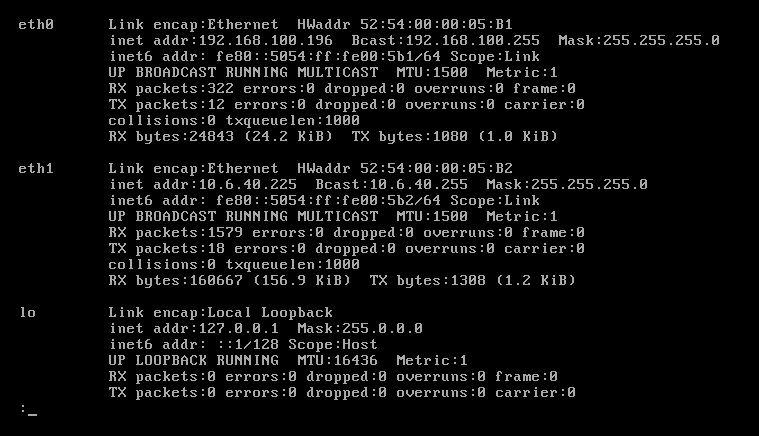
\includegraphics[width=.65\linewidth]{screenshots/ifconfig/ifconfig.png}
}
\medskip
     \\Fig. 1: Interfaces de red en máquina con CentOs server.
\end{minipage}
\newpage
\subsection{Instalacion httpd}
Para iniciar la instalación del servidor, abrimos una consola y ejecutamos \textbf{yum install httpd}, de esta forma comenzamos la descarga de archivos y paquetes necesarios, y la instalación propiamente tal.

\begin{minipage}[t]{\linewidth}
    \raggedright
	    \adjustbox{valign=t}{
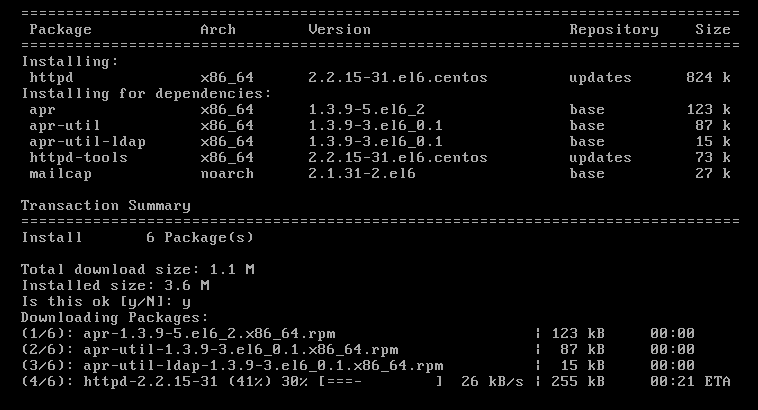
\includegraphics[width=.65\linewidth]{screenshots/httpd-install/descargando-paquetes.png}
}
\medskip
     \\Fig. 2: Descarga de paquetes necesarios para la instalación.\\
\end{minipage}

\begin{minipage}[t]{\linewidth}
    \raggedright
	    \adjustbox{valign=t}{
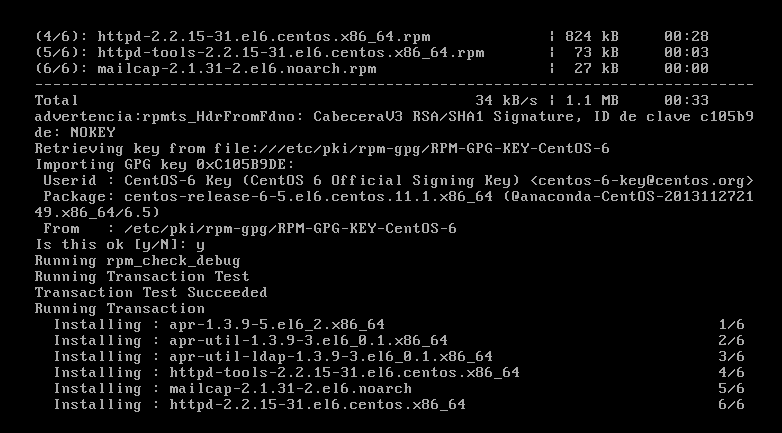
\includegraphics[width=.65\linewidth]{screenshots/httpd-install/instalando.png}
}
\medskip
     \\Fig. 3: Instalación del servidor en curso.\\
\end{minipage}

\begin{minipage}[t]{\linewidth}
    \raggedright
	    \adjustbox{valign=t}{
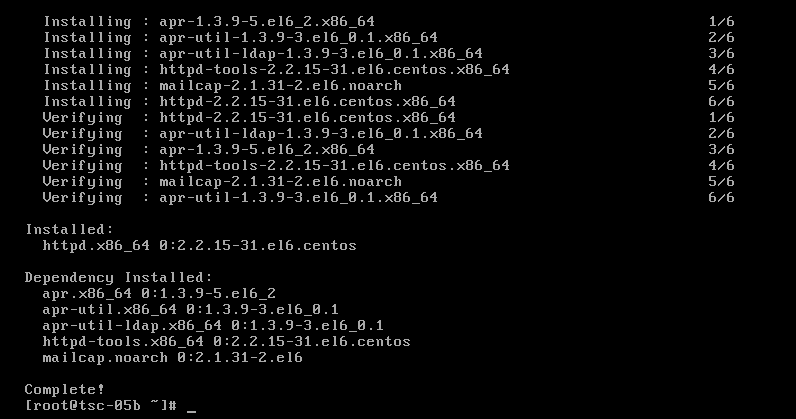
\includegraphics[width=.65\linewidth]{screenshots/httpd-install/terminado.png}
}
\medskip
     \\Fig. 4: Instalación del servidor finalizada.\\
\end{minipage}

\subsection{Verificación httpd}
Para comprobar que todo está en orden posterior a la instalación, ejecutamos \textbf{yum info httpd}, esto nos da información acerca del programa.\\

\begin{minipage}[t]{\linewidth}
    \raggedright
	    \adjustbox{valign=t}{
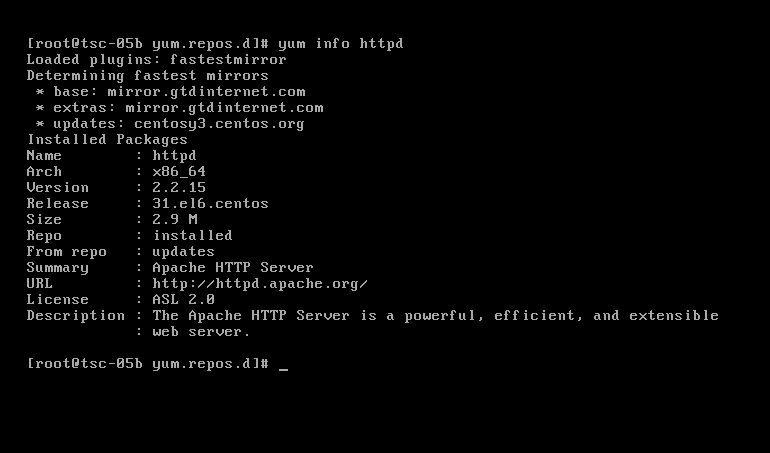
\includegraphics[width=.65\linewidth]{screenshots/httpd-install/yum-info-httpd.png}
}
\medskip
     \\Fig. 5: Comprobación que el paquete ha sido instalado.\\
\end{minipage}

\subsection{Configuración httpd}
El siguiente paso consiste en configurar la partida del servidor, esto se hace a través de un comando \textbf{chkconfig httpd on}. Notar en la siguiente figura que para la fila de httpd, los \textit{demonios} 1-5 están en \textit{activo}, por lo que sólo resta levantar el servicio.\\

\begin{minipage}[t]{\linewidth}
    \raggedright
	    \adjustbox{valign=t}{
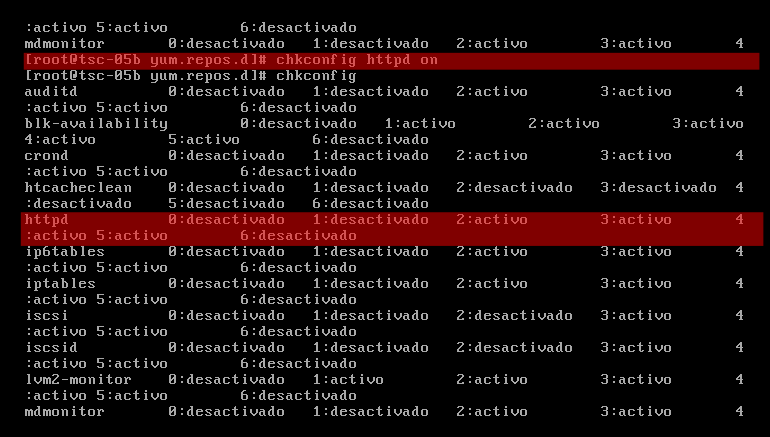
\includegraphics[width=.65\linewidth]{screenshots/httpd-run/chkconfig-httpd-on.png}
}
\medskip
     \\Fig. 6: Configuración de partida.\\
\end{minipage}
\newpage

\subsection{Puesta en marcha y prueba}
Para levantar el servicio servidor, ejecutamos \textbf{service httpd start}, de esta forma nuestro servidor se encuentra virtualmente arriba, con lo que sólo faltaría otro par de ajustes para finalizar.\\

\begin{minipage}[t]{\linewidth}
    \raggedright
	    \adjustbox{valign=t}{
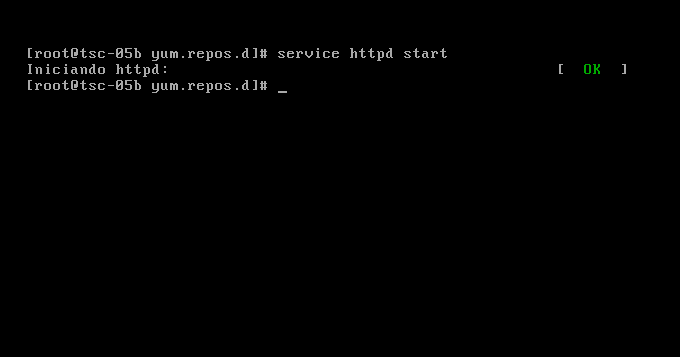
\includegraphics[width=.65\linewidth]{screenshots/httpd-run/service-httpd-start.png}
}
\medskip
     \\Fig. 7: Levante de servicios.\\
\end{minipage}

Ahora bien, para comprobar mediante comandos que el servicio efectivamente esté corriendo, ejecutamos \textbf{service httpd status}, lo que arroja el siguiente resultado:\\

\begin{minipage}[t]{\linewidth}
    \raggedright
	    \adjustbox{valign=t}{
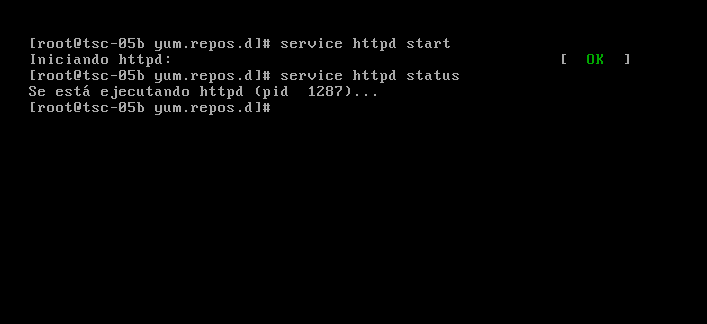
\includegraphics[width=.65\linewidth]{screenshots/httpd-run/service-httpd-status.png}
}
\medskip
     \\Fig. 8: Estado del servicio instalado.\\
\end{minipage}
\newpage
\subsection{Permisos de archivos}
Es necesario verificar el nivel de acceso a archivos desde el sistema operativo, para ello ejecutamos \textbf{getenforce}, lo que comprueba el estado y nos arroja \textit{Enforcing}, con lo que tenemos que cambiar el estado a \textit{Permissive} mediante \textbf{setenforce permissive}.\\

\begin{minipage}[t]{\linewidth}
    \raggedright
	    \adjustbox{valign=t}{
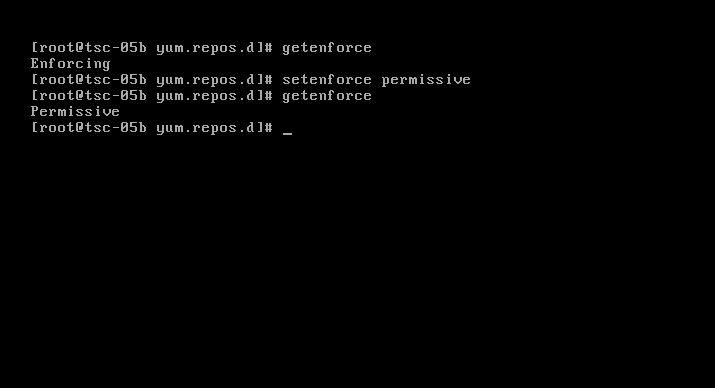
\includegraphics[width=.65\linewidth]{screenshots/permissions/set-permissive.png}
}
\medskip
     \\Fig. 9: Nivel de acceso a archivos desde el SO.\\
\end{minipage}

\subsection{Configuración firewall}
Además, es necesario añadir una regla para el \textit{firewall}, de manera de aceptar conexiones al puerto 80. Esto se hace a través de la edición del archivo \textit{iptables}, el que es posible editar desde consola mediante \textbf{vi /etc/sysconfig/iptables}.\par
El archivo editado debería quedar se la siguiente forma:\\

\begin{minipage}[t]{\linewidth}
    \raggedright
	    \adjustbox{valign=t}{
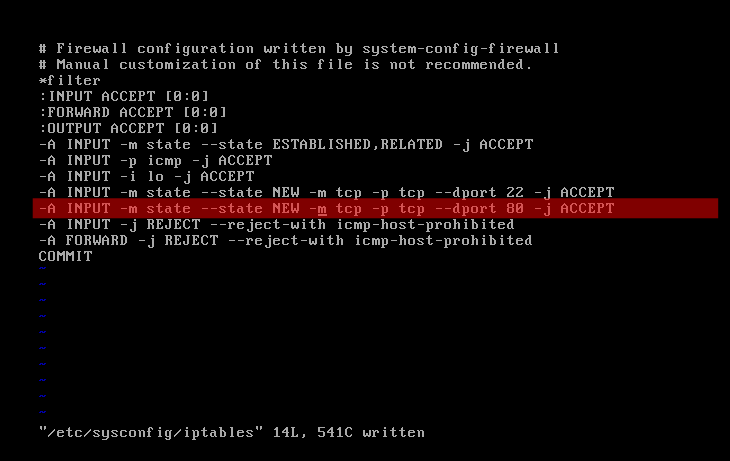
\includegraphics[width=.65\linewidth]{screenshots/iptables-config/vi-iptables-port-80-enabled.png}
}
\medskip
     \\Fig. 10: Configuración de firewall.\\
\end{minipage}
\newpage
Posterior a esto, para que los cambios surjan efecto es preciso reiniciar el sistema o simplemente reiniciar el servicio. Se opta por esto último, lo que se lleva a cabo con \textbf{service iptables restart}.\\

\begin{minipage}[t]{\linewidth}
    \raggedright
	    \adjustbox{valign=t}{
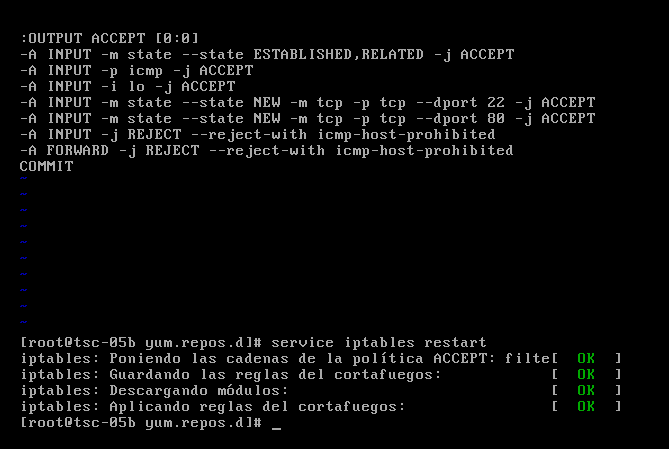
\includegraphics[width=.65\linewidth]{screenshots/iptables-config/iptables-restart.png}
}
\medskip
     \\Fig. 11: Reinicio servicio firewall.\\
\end{minipage}

Ahora con todo esto configurado, se debería ser capaz de conectar al servidor desde otra máquina, lo que se muestra en la próxima sección.

\subsection{Conexión al servidor mediante Telnet}
\textit{Telnet} permite conectarse a un servidor desde otra máquina de forma remota. Su uso ha sido descontinuado dada su baja seguridad, sin embargo, se utiliza en esta experiencia con fines experimentales.\par
Dado que por defecto \textit{Telnet} no viene con la versión de CentOs instalada, debemos instalarlo manualmente mediante \textbf{yum install telnet}:\\

\begin{minipage}[t]{\linewidth}
    \raggedright
	    \adjustbox{valign=t}{
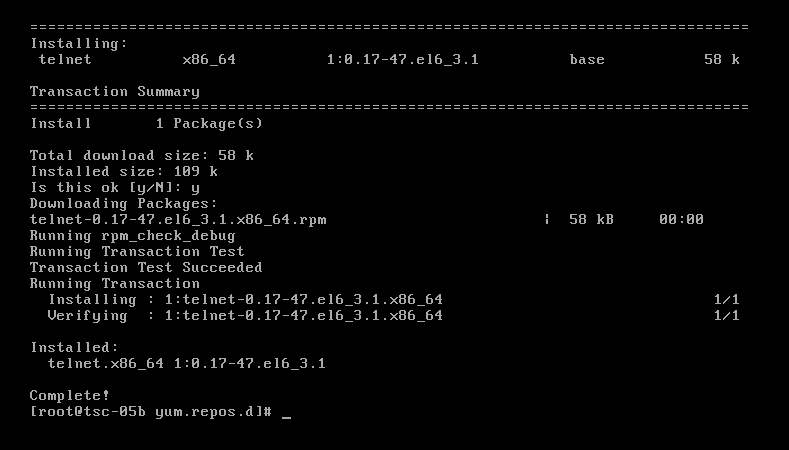
\includegraphics[width=.65\linewidth]{screenshots/telnet-install/telnet-instalacion-completa.png}
}
\medskip
     \\Fig. 12: Instalación \textit{Telnet} finalizada.\\
\end{minipage}
\newpage
Ahora, con un simple \textbf{telnet localhost 80} y luego escribiendo \textbf{GET /} se descarga la página html por defecto en formato texto.\\

\begin{minipage}[t]{\linewidth}
    \raggedright
	    \adjustbox{valign=t}{
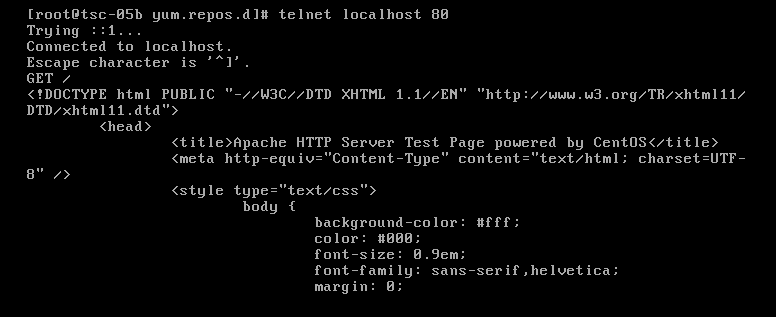
\includegraphics[width=.65\linewidth]{screenshots/communication/telnet-get-80.png}
}
\medskip
     \\Fig. 13: Página html en formato de texto plano, obtenida mediante \textit{Telnet} en la misma máquina.\\
\end{minipage}

De forma análoga, también podemos realizar esto desde la máquina anfitrión, teniendo en consideración que ahora debemos ingresar la IP de la máquina mínima en lugar de localhost, o sea, debemos ingresar \textbf{telnet 10.6.40.225 80}\\

\begin{minipage}[t]{\linewidth}
    \raggedright
	    \adjustbox{valign=t}{
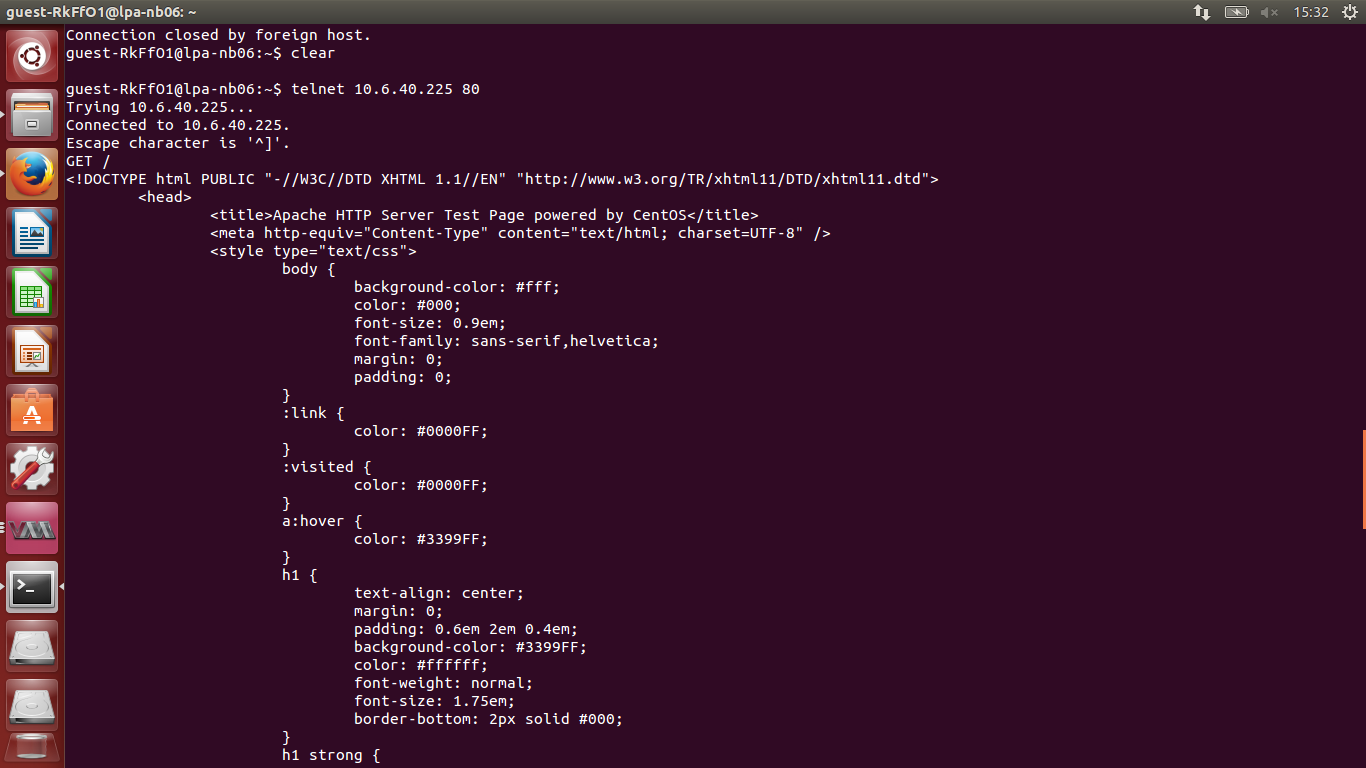
\includegraphics[width=.65\linewidth]{screenshots/communication/get-to-min-from-host.png}
}
\medskip
     \\Fig. 14: Página html en formato de texto plano, obtenida mediante \textit{Telnet} en máquina anfitrión.\\
\end{minipage}
\newpage
\subsection{Conexión al servidor mediante browser}
Finalmente, se desea conectar al servidor mediante un explorador web con interfaz gráfica. Nuevamente desde la máquina anfitrión abrimos un navegador cualquiera, e ingresamos en la barra de direcciones la dirección IP del servidor, o sea, \textbf{10.6.40.225}, dando como resultado la página por defecto de Apache.\\

\begin{minipage}[t]{\linewidth}
    \raggedright
	    \adjustbox{valign=t}{
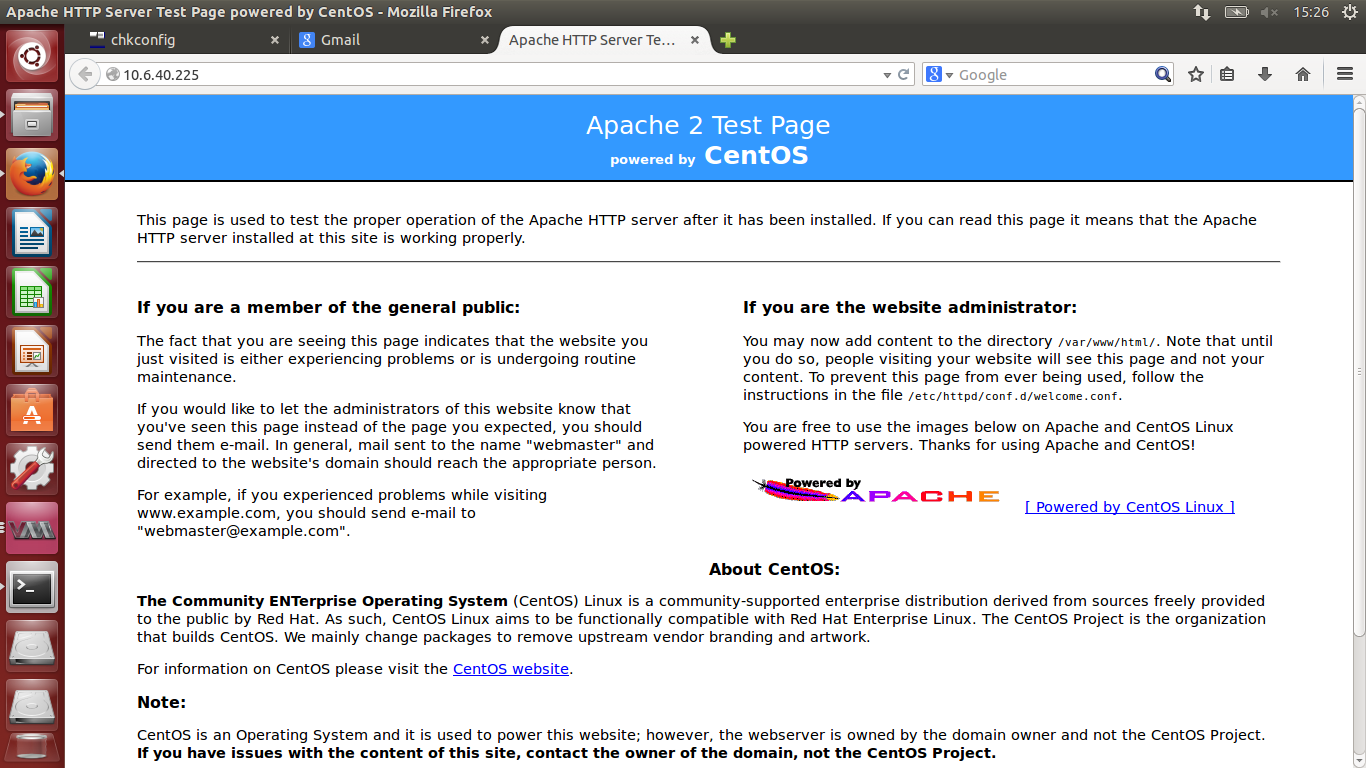
\includegraphics[width=.65\linewidth]{screenshots/communication/host-browser-to-min.png}
}
\medskip
     \\Fig. 15: Página web obtenida mediante \textit{browser} en máquina anfitrión.\\
\end{minipage}

\section{Conclusión}
Se logró instalar de forma satisfactoria el servidor web Apache httpd, además de configurarlo únicamente mediante línea de comandos, lo que en un principio parecería complejo, sin embargo, los cambios que deben hacerse son pocos y se espera que siguiendo esta guía, cualquier persona sea capaz de hacerlo.

\end{document}
